\documentclass[a4paper,12pt]{article}  % 文書の種類を指定

% --- パッケージの読み込み（便利機能を追加） ---
\usepackage[utf8]{inputenc}   % UTF-8文字コードを使用
\usepackage[T1]{fontenc}      % 出力フォントのエンコード
\usepackage{amsmath,amssymb}  % 数式関係
\usepackage{graphicx}         % 画像を挿入
\usepackage{siunitx}          % 単位付き数値（例: \SI{10}{\meter}）
\usepackage{caption}          % 図表キャプションをカスタマイズ
\usepackage{geometry}        % 余白設定
\usepackage{comment}
% \usepackage{hyperref}
\usepackage[colorlinks=true, linkcolor=blue]{hyperref}
\usepackage{indentfirst}
\usepackage{listings}
\usepackage{xcolor}
\renewcommand{\lstlistingname}{Script}
\lstset{
  % basicstyle=\ttfamily\footnotesize,
  basicstyle=\ttfamily\footnotesize\lst@ifdisplaystyle\else\raggedright\fi,
  numbers=left,
  numberstyle=\tiny,
  frame=single,
  breaklines=true,
  showstringspaces=false,
}      % Indent the first paragraph of each section
\geometry{margin=25mm}

% --- タイトルなど ---
\title{Instruction of Python API for Leica AT 401}
\author{Shohta Takami}
% \date{\today}

% --- 本文開始 ---
\begin{document}

\maketitle
\begin{comment}
\section{Introduction}
Leica Laser Tracker AT401 deploys TCP/IP socket connection for communication even when you use official software developped by Leica.
I needed to develop a method to operate Leica Laser Tracker by purely Python dependent way in order to integrate other DAQ systems such as the Hall probe and the motor control.
This is a document about how to use pure Python API to operate Leica Laser Tracker AT401.
You can download the program here (\url{https://github.com/shohty/LeicaAT401_MIT}).
The programs actually used in the operation of Leica AT401 are shown in the list below.
\begin{center}
\begin{minipage}{0.5\textwidth}  % 全体幅を少し狭く
  \centering
  \captionof{table}{Scripts for Leica AT401 operation}
  \label{tab:script_list}
  \begin{enumerate}
    \item \texttt{"CESAPI/command.py"}
    \item \texttt{"CESAPI/packet.py"}
    \item \texttt{"CESAPI/connection.py"}
    \item \texttt{"shohta/MeasDemo.py"}
  \end{enumerate}
\end{minipage}
\end{center}

\section{API structures}
There's a header file named \texttt{"ES\_C\_API.h"} in the directory \texttt{"include/"}.
If you want to get it officially, you should make a contact with Hexagon customer support (\url{https://portable-mi.hexagon.com/}).
The difinitions of commands and the data structure for each command are written in this header file.
% They are basically defined by numbers.
The contents of the header file is written at the first few hundreads lines of \path{"CESAPI/packet.py"} because the original header file is written in C-style, which is not readable for Python.
% In \texttt{"CESAPI/packet.py"}, the classes for all commands are defined.
All classes are named after the command in the header file.
The classes to send the command are suffixed with "CT" after its command name.
The classes to store the response are suffixed with "RT" as well as ones to send.
Each classes have functions to pack the command to the binary or unpack the binary response.
\end{comment}


\section{API structures}
\subsection{The Concept}
\begin{figure}[h]
    \centering
    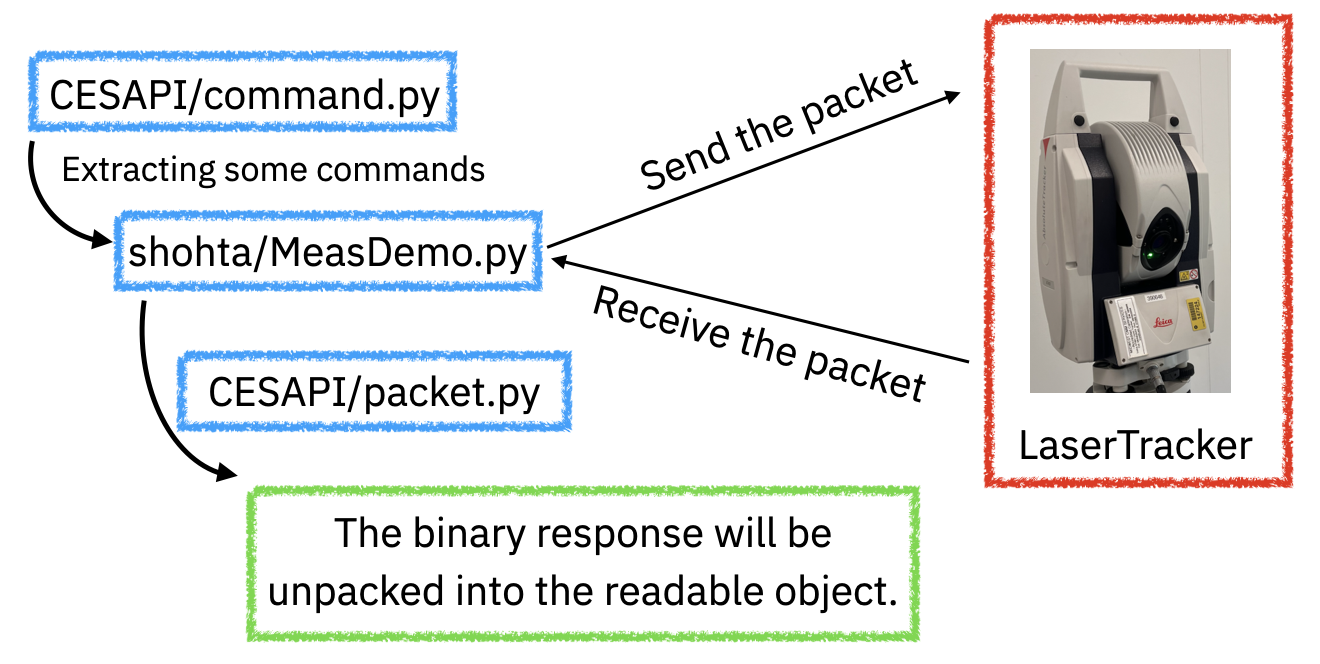
\includegraphics[width=0.7\linewidth]{figure/structure.png}
    \caption{The general flow}
    \label{fig:structure}
\end{figure}
 The communication with Leica AT4xx will be conducted by binary packet protocol.
You have to send and read the binary packet.
The structure of the binary for each command is defined in the header file \path{"Include/ES_C_API_Def.h"}.
If you want to get the latest header file, you should make a contact with Hexagon customer support (\url{https://portable-mi.hexagon.com/}).

Figure.{\ref{fig:structure}} shows the conceptual flow of this API.
\path{"MeasDemo.py"} is written by myself extracting commands from \path{"command.py"}.
\path{"packet.py"} provides functionality to convert numerically-defined command IDs into binary format, and to parse returned binary data into objects.
command.py is responsible for sending the binaries generated by packet.py over TCP/IP and receiving binaries via TCP/IP.
Then, the response from the laser tracker can be read by accessing the relevant instance variables of the returned object.

\subsection{ When you want to change the header file}
\path{"Include/ES_C_API_Def_clean.h"} is the modified version of the header file to compatible for Python.
When you want to use another header file, you have to regenerate \path{"packet.py"} and \path{"command.py"}.
The original header file \path{"Includes/ES_C_API_Def.h"} is written in C-style, which is not readble for Python.
The file \path{"ES_C_API_Def_clean.h"} is modified to make it compatible for Python.
Unnecessary macros, typedefs, and unused structures have been removed, and overly nested definitions were flattened.
Function and structure names were preserved, but formatting and alignment were adjusted to improve readability and automatic parsing by the Python generator script.
It is assumed in the comments in the original header file that you will not have to switch the header file as long as you use AT4xx series.

\section{The method to use commands}
\begin{lstlisting}[caption={The definition of the class for GetTrackerInfo}, label={lst:gettkrinfo} ]
class GetTrackerInfoRT(object):
  def __init__(self):
    self.packet = b''
    self.__packet_size = 164
    self.__sizes = [148]
    self.__formats = [('<I 64s i i i i i d d d i i d d I i i ')]
    self.packetInfo = BasicCommandRT()
    self.packetInfo.packetHeader.lPacketSize = self.__packet_size
    self.packetInfo.packetHeader.type = ES_DT_Command
    self.packetInfo.command = ES_C_GetTrackerInfo
    self.trackerType = int(0)  
    self.cTrackerName = b''  
    self.lSerialNumber = int(0)
    self.lCompensationIdNumber = int(0)
    self.bHasADM = int(0)
    self.bHasOverviewCamera = int(0)
    self.bHasNivel = int(0)
    self.dNivelMountOffset = float(0)
    self.dMaxDistance = float(0)
    self.dMinDistance = float(0)
    self.iMaxDataRate = int(0)
    self.iNumberOfFaces = int(0)
    self.dHzAngleRange = float(0)
    self.dVtAngleRange = float(0)
    self.accuracyModel = int(0)  
    self.iMajLCPFirmwareVersion = int(0)
    self.iMinLCPFirmwareVersion = int(0)
\end{lstlisting}
\begin{lstlisting}[caption={The structure of the binary for GetTrackerInfo defined in the header file}, label={lst:gettkrinfo_header} ]
struct GetTrackerInfoRT
{
    struct BasicCommandRT    packetInfo;
    enum ES_LTSensorType     trackerType;
    unsigned short           cTrackerName[32];         
    long                     lSerialNumber;
    long                     lCompensationIdNumber;      
    ES_BOOL                  bHasADM;
    ES_BOOL                  bHasOverviewCamera;
    ES_BOOL                  bHasNivel;
    double                   dNivelMountOffset;
    double                   dMaxDistance;               
    double                   dMinDistance;               
    int                      iMaxDataRate;              
    int                      iNumberOfFaces;
    double                   dHzAngleRange;              
    double                   dVtAngleRange;
    enum ES_TrkAccuracyModel accuracyModel;
    int                      iMajLCPFirmwareVersion;
    int                      iMinLCPFirmwareVersion;
};
\end{lstlisting}
Here, I explain how to use "GetTrackerInfo" command as an example, which is for retrieving the basic infomation of the laser tracker. 
First, you have to make an instance of all commands from \path{"CESAPI/command.py"}.
% Second, get the object you want by calling the function you want to use ("GetTrackerInfo" for this example).  
Each function in \path{"CESAPI/command.py"} also includes the feature to send the packet by the function "execute".
So, you will get the object corresponding to the function as returned value, after executing the function.
The structure of each returned object is defined in the class namely suffixed with "RT" to the name of the command you used (shown as Script.\ref{lst:gettkrinfo}).
You can also look up to \path{"Includes/ES_C_API_Def.h"}, which \path{"CESAPI/command.py"} is originated from.
Here is the example flow of access to returned object.
\begin{lstlisting}[caption={The flow to get the tracker's name}]
command = CommandSync() #make an instance of command
tkrinfo = command.GetTrackerInfo()
tkrname = tkrinfo.cTrackerName
print(f"{tkrname}")
There is one exception for this naming convention.
When you measure the coordinate, you. have to use 
\end{lstlisting}
\subsection{The command to take coordinates}
Regarding of the command to take coordinates, the naming convention explained above will be different.
When you measure the coordinate of the pointing reflector, you would have to use command named "StartMeasurement".
For this command, the returned object will differ depnding on the status.
If the tracker returns some error, the returned object will be "StartMeasurementRT".
When the command works successfully, the object named "SingleMeasResultT" will be returned (shown in Script.\ref{lst:SingleMeasResultT}).
So you should look up to the structure of "SingleMeasResultT" when you use "StartMeasurement" to measure the coordinate.
\begin{lstlisting}[caption={SingleMeasResultT is returned as a response to "StartMeasurement"}, label={lst:SingleMeasResultT}]
struct SingleMeasResultT
{
    struct ReturnDataT packetInfo;
    enum ES_MeasMode   measMode;
    ES_BOOL            bIsTryMode;
    double             dVal1;
    double             dVal2;
    double             dVal3;
    double             dStd1;
    double             dStd2;
    double             dStd3;
    double             dStdTotal;
    double             dPointingError1;
    double             dPointingError2;
    double             dPointingError3;
    double             dAprioriStd1;
    double             dAprioriStd2;
    double             dAprioriStd3;
    double             dAprioriStdTotal;
    double             dTemperature;
    double             dPressure;
    double             dHumidity;
};
\end{lstlisting}

dVal1 to dVal3 corresponds to the coordinates.
The numbering follows the same ordering of coordinates as described in the documentation (\path{TPI3.0_ProgrammersManual.pdf}).
Basically, I applied the spehrical counter-clockwise system in Figure.\ref{fig:coordsys} following EMMA.
In this case, dVal1 is H, dVal2 is V, dVal3 is D. 
\begin{figure}[h]
    \centering
    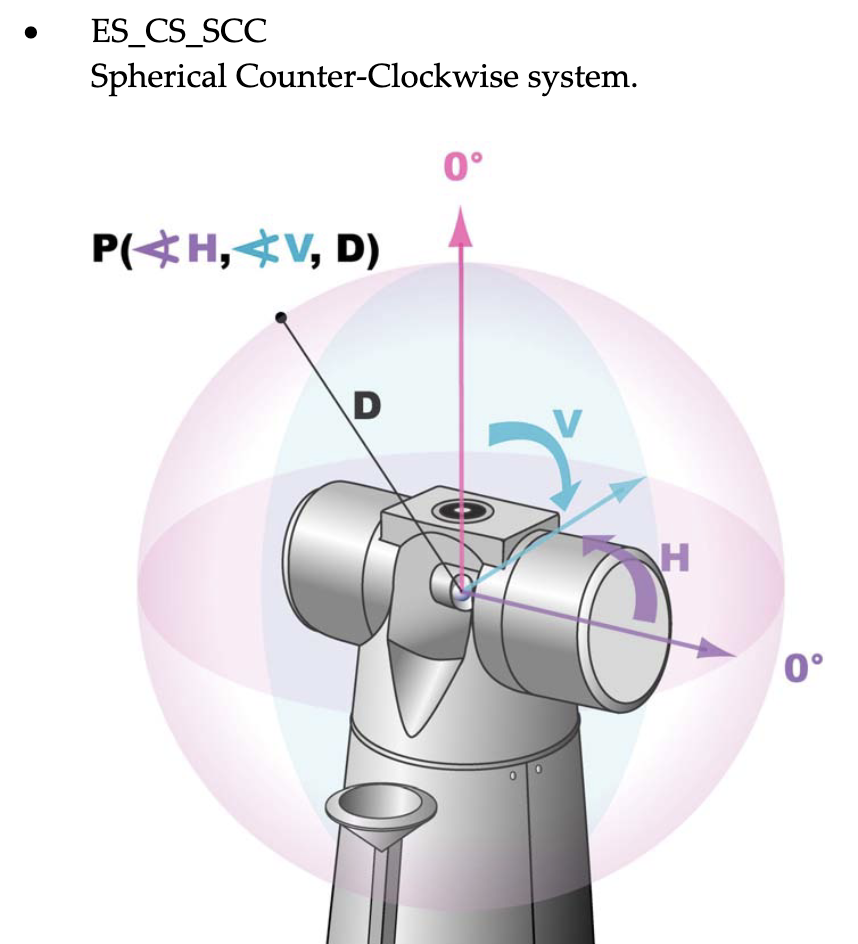
\includegraphics[width=0.7\linewidth]{figure/coordsys.png}
    \caption{Spherical Counter-Clockwise System}
    \label{fig:coordsys}
\end{figure}
\section{Changing configurations}
\begin{center}
\begin{minipage}{0.5\textwidth}  % 全体幅を少し狭く
  \centering
  \captionof{table}{The configuration list}
  \label{tab:config}
  \begin{enumerate}
    \item Measurement mode
    \item Weather monitor
    \item Orientation Params
    \item Transformation Params
    \item Units
    \item Coordinate system type
  \end{enumerate}
\end{minipage}
\end{center}

Table.\ref{tab:config} shows the lists of configurations.
You have to set the configuration actively before measurement.
In this section, I explain how to modify the settings by using the unit-system configuration as an example.
\begin{lstlisting}[caption={The scripts to change configuration}, label={lst:changeunit}]
def set_units():
    units = SystemUnitsDataT()
    units.lenUnitType = ES_LU_Millimeter     
    units.angUnitType = ES_AU_Radian         
    units.tempUnitType = ES_TU_Fahrenheit  
    units.pressUnitType = ES_PU_InHg        
    units.humUnitType = ES_HU_RH              
    command.SetUnits(units)
    print(f'Units set successfully')
\end{lstlisting}

Script.\ref{lst:changeunit}, extracting from \path{"shohta/MeasDemo.py"} shows how to change the configuration of units system.
The way to change configuration is all the same.
First, you have to make an instance of configuration (pick right one, easily estimated from its name).
Second, you just have to define each instance variables to configuration as you like.
The difinition of units are defined in \path{"Include/Enum.h"} and those of other configurations are defined in \path{"Include/ES_C_API_Def.h"}.
You can also find the definition of these configuration in the first few hundreads of lines in \path{"CESAPI/packet.py"}.
After creating the instance of your configuration as above, you can apply the configuration by the \path{"Setxxx"} function.

\section{Practical use of MeasDemo.py}
\path{"shohta/MeasDemo.py"} is the script I actually used.
It imports \path{"CESAPI/connection.py"} and \path{"CESAPI/command.py”}, \path{"CESAPI/packet.py}.
I organized the functions according to the calling sequence.
The main function is for the repeated measurement explained below.
\subsection{TCP/IP Connection}
First, you have to connect to the laser tracker.
The default address is \path{"192.168.0.2"}, and the port number is \path{700}.
You have to make an instance of the class in \path{CESAPI/connection.py}.
Then, connect to the laser tracker using the function in this class.
After successfully connection, you have to input the instance of connection to the object \path{CommandSync} in \path{"CESAPI/comand.py"}.
\begin{lstlisting}[caption={The command to make a connection}, label={lst:conn}]
conn = Connection()
conn.connect(host='192.168.0.2', port=700)
ommand = CommandSync(conn)
\end{lstlisting}

\subsection{Before measurement}
You have to set the configurations in Table.\ref{tab:config} as I explained above before the measurement.
At that moment, I followed the EMMA's configuration.
We may have to figure out the appropriate configuration.

You have to initialize before measurement (The second command in Table.\ref{tab:setting}).
% I am not sure whether the order of setting the configurations does matter or not.
Lastly, you have to execute \path{"set_system_setting"} to apply every configuration so far.
"1" means "Apply", and "0" means "Not Apply".  
\begin{center}
\begin{minipage}{0.5\textwidth}  % 全体幅を少し狭く
  \centering
  \captionof{table}{Commands to set configurations}
  \label{tab:setting}
  \begin{enumerate}
    \item \path{set_units()}
    \item \path{initialization}
    \item \path{set_weathermonitor()}
    \item \path{set_TransformationParam()}
    \item \path{set_OrientationpParam()}
    \item \path{set_measurement_mode()}
    \item \path{set_CoordinateSystemType(7)}
    \item \path{set_system_setting()}
  \end{enumerate}
\end{minipage}
\end{center}
% Table.\ref{tab:config} shows the list of functions in \path{CESAPI/MeasDemo.py} to set the configurations.
After all these setting, you will be ready to operate the tracker.

\subsection{The operation of the laser tracker}
The operations I needed were just "pointing the laser to arbitary coordinate" and "measuring the coordinates".

The function, \path{"go_to_position"}, sends the command to point the laser to the arbitary point.
The values of 3 coordinates as you configured is required as arguments.
According to \path{"TPI3.0_ProgrammersManual.pdf"}, you have to input \path{"True"} to the fourth argument \path{"bUseADM} because AT4xx series has ADM (Absolute Distance Meter).
The tracker will automatically do the spiral search if it can't find any reflector at the input coordinate.

The function, \path{"point_measure"}, sends the command to measure the coordinate and repeat the measurement input times.
In this function, the measured data and measurement information are recorded to the csv file and root file which contains TTree object as a log.
Table.\ref{tab:csv} shows columns of this log file.
\begin{center}
\begin{minipage}{0.5\textwidth}  % 全体幅を少し狭く
  \centering
  \captionof{table}{The list of the log file}
  \label{tab:csv}
  \begin{enumerate}
    \item coordinate system type
    \item point name
    \item measurement id
    \item measurement mode
    \item date
    \item time
    \item coordinates
    \item standard deviations of each coordinate
    \item the total standard deviation
  \end{enumerate}
\end{minipage}
\end{center}
The coordinate system type will be recorded by the number defined in the header file or \path{"packet.py"}.
The measurement id specifies the order of the measurement in a series of repeated measurements.
(I regret not adding the environmental information such as the temperature even though you can easily access them as the measured coordinates.)
I tried 100-time repeated measurement and it took roughly 30 minuetes.
One unexpected error is that measurements sometimes start to fail.
I could not identify why this happens, but the configuration for the weaather monitor somehow was changed to \path{"ReadOnly"} every time; nevertheless it should be \path{"ReadandCalculateRefractions"}.










\end{document}
